\section{Literature Review}

% Talk about the meaning and history of fuzzing

\begin{figure}[!b]
    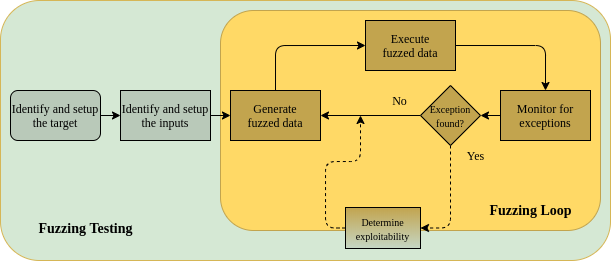
\includegraphics[width=\textwidth]{Chapter2/FuzzingPhases.png}
    \centering
    \caption{Fuzzing phases}
    \label{fig:fuzz_phases}
\end{figure} 

% ! It would be good to mention that the meaning of program, application and executable are all the same

Sutton et al. \cite{sutton2007fuzzing} defined the procedure of fuzz testing, as shown in Figure \ref{fig:fuzz_phases}:
\begin{enumerate}
    \item Generally speaking, the first stage is to identify the target. A target may be a software or a combination of both software and hardware \cite{song2019periscope}. The targeted software may be the software itself, or any part of the software, for instance, a library or an API. In the rest of this article, our target is software.
    
    \item To execute the target program, we need to specify how the program parses the inputs. For instance, the target program may take several command-line arguments as the input, or the arguments are file locations for reading data. Environmental variables, file formats, and any other variables that may change the program's execution are all considered an input, and a fuzzer should choose them for the execution of the target program. In any case, the fuzzer needs to know the data that would cause a vulnerability. 
    
    A fuzzer may need a set of seeds for initialization. This set could be empty, and a fuzzer without any sample inputs may find some valid files out of thin air \cite{out_of_thin_air} that are acceptable by the target program.
    
    \item The generation of fuzzed data is the beginning of the fuzz testing loop. The target program needs a queue of inputs for testing the execution. New inputs are generated either by a dumb mutation of the content of the input, or by generating new content based on some heuristics. The prior procedure is part of a mutation-based fuzzing, and a generation-based fuzz testing uses the later. Waffle is a mutation-based fuzz testing platform based on AFL. In \autoref{chap:ch3}, we will discuss more about how a mutation-based dumb fuzzer works intelligently.

    \item A fuzzer takes the processed inputs and executes the target program using the provided inputs. Depending on the resources needed for the execution of the target program, this stage can be the bottleneck for the procedure of fuzzing. Generally, the output of this stage is any detected misbehavior during the execution of inputs. 
    
    \item If an exceptional event happens during the execution of the program that prevents the program from exiting successfully, we say an exception has occurred. It is expected for a program to finish it's execution by returning a success value, 0 for most machines. If any value other than the success value (0) is returned,  These exceptions are the vulnerabilities that may be exploitable and may cause security problems. Handling an exception properly and pinpointing the input (or probably part of the content of the input) responsible for the exception is the primary purpose of this stage of fuzz testing. 
    
    \item A vulnerability may be harmless! Suppose we find an exception (vulnerability) in a module not handled within the program, and the operating system catches it. If another program uses this module, and the program is first validating the input for the module, then the domain of inputs for this module is constrained and filtered by the program, and the vulnerability may never occur. If we can find an exploitable vulnerability, the fuzzer must detect it and report it as an exploitable vulnerability. The generation phase may need this report for later usage.

\end{enumerate}

\vspace{1.5\baselineskip}

% Different methods of fuzzing such as \textit{pregenerated test-cases}, \textit{random generation} and \textit{mutation testing} are common in different fuzzers. Fuzzers may fuzz the \textit{environmental variables}, \textit{file format} or \textit{content of the input} and may target \textit{remote targets}, \textit{network} or any \textit{programs} executable in a machine; the targets may be software or hardware.  A neural network is also fuzzed as a target program in TensorFuzz \cite{odena2018tensorfuzz} and DeepHunter \cite{xie2018coverage} to investigate the flaws of the network.



% Blackbox fuzzer

The introduced fuzzer by Miller \cite{miller1990empirical} was of the very first naive blackbox fuzzer targeting a collection of Unix utilities, on different Unix versions. It runs the fuzzing for different lengths of inputs for each utility (of the total 88 utilities) and expects a \textbf{crash}, \textbf{hang}, or a \textbf{succeed} after the execution of the program. The generation of inputs is by the mutation of the content of the inputs, and the target program is a blackbox for the fuzzer. As a result, this fuzzer is a mutation-based blackbox fuzzer.


\vspace{1.5\baselineskip}

A blackbox fuzzer randomly generates a different stream of inputs and does not decide how to choose those generations to enhance the performance of the fuzzer. Another downside of this fuzzer (and other blackbox fuzzers) is when the program faces some branches with magic values, constraining the variable to a specific set of values; the fuzzer has to apply the exact values for the constraining statement which may have a very low probability - it is almost impossible to generate a specific 1 KB string of bytes by chance. Nevertheless, when the target application is known, the performance of the blackbox fuzzing technique can be increased drastically. In \cite{banks2006snooze} and \cite{gascon2015pulsar} a set of network protocols are fuzzed as blackbox. Any application on the web may be considered as a blackbox program as well, so as \cite{doupe2012enemy} and \cite{duchene2012xss} have targeted web applications and found ways to attack some the websites, looking for different vulnerabilities, such as XSS.

% Whitebox fuzzers
\vspace{1.5\baselineskip}

SAGE, a whitebox fuzzer was developed as an alternative to blackbox fuzzing, to cover the lacks of blackbox fuzzers \cite{godefroid2012sage}. A fuzzer is a whitebox fuzzer if we have the source code of the target program, and the fuzzer can use the information within the source code. With the benefit of having the source code and internal knowledge for fuzzing, a whitebox fuzzer can leverage symbolic constraints for symbolic analysis to solve the constraints in the program \cite{cadar2011symbolic}. It can also use dynamic, and concolic execution \cite{stephens2016driller} and use taint analysis to locate the regions of seed files influencing values used by program \cite{ganesh2009taint}; whitebox fuzzing can also find the grammar for parsing the input files without any prior knowledge \cite{godefroid2008grammar}. These techniques help in finding code coverage and a more intelligent search for vulnerabilities.

% Greybox fuzzers

% TODO:    Whitebox fuzzing must use the information in source code! For instance, if we are benefiting something from source code, that is whitebox. If we are not doing that, like what AFL does during the compilation time, just putting a unique marker in each basic-block, and using that information for later investigations. This is a true Greybox fuzzing! LLVM and QEMU are both doing a greybox thing ;)

% !        Let's ignore the colors! Don't consider the w/b/g-box fuzzing. Instead, let's think about this: Are we using the knowledge of the creator of the program for our fuzzing purposes? If we are doing that, then that's one of the groups of fuzzers, like the graybox fuzzing we were talking about before. I suppose this non-logical knowledge of the program has an important role in distinguishing the fuzzers from each other :D

\vspace{1.5\baselineskip}

Greybox fuzzing resides between whitebox and blackbox fuzzing, as we only have partial knowledge about the internals of the target program. We do not have the source code, but we have some knowledge about the program (for instance, we have the binary file), and as a result, we have the instructions for the program, which can be helpful for the fuzzing. A handy feature for an execution is the code coverage of the run. A coverage-based greybox fuzzer keeps track of the different inputs with different coverages and may generate inputs for the next generations based on the new code coverages found in each iteration. To detect the coverage, we need an instrumentation \cite{liang2018fuzzing} that we will explain more in section \nameref{instrumentation}. 

% Coverage-based fuzzers

\vspace{1.5\baselineskip}

Coverage-based fuzz testing benefits from instrumentation for discovering the parts of the (binary) code that are covered during the executions. Some criteria, such as data coverage, statement coverage, block coverage, decision coverage, and path coverage, can be used to investigate the overall code coverage. \cite{yang2009survey} Bohme et al. \cite{bohme2017coverage} introduced a coverage-based greybox fuzzer that extends AFL and benefits from the Markov Chain model. The fuzzer looks for the paths that were covered using seeds, and when a new path is seen, it is stored accordingly. Then it reports a probability that after fuzzing an input with path \textit{i}, it generates an input with path \textit{j}. The fuzzer chooses a new collection of seeds to fuzz based on the energies assigned to each seed; it generates more inputs from a seed with higher energy.

In another article by Bohme et al. \cite{bohme2017directed}, they introduce their directed fuzzing by the idea of checking the code-coverage for providing inputs that guide the program execution toward some targeted locations. Some of the applications of such fuzzing approach are patch testing and crash reproduction, which have different use cases compared to non-directed coverage-based fuzzers.

\vspace{1.5\baselineskip}

% Performance fuzzers
% TODO: Check if the claims are all true

The types of vulnerabilities that a fuzzer is involved with may be different from other fuzzers. For example, AFL looks for crashes or hangs by selecting and mutating the inputs, and at the same time, it considers the code coverage, size of the input, and the execution time of the target program. PerfFuzz \cite{lemieux2018perffuzz} is another greybox fuzzer based on AFL, which aims to generate inputs for executions with higher execution time, while using most of the features of AFL in exploring for more coverage. PerfFuzz counts how many times each of the edges of the control flow graph (CFG) is executed. Using SlowFuzz \cite{petsios2017slowfuzz}, we can consider any type of resource as a feature to detect the worst-case scenarios (inputs) for a given program. In another project based on AFL, Memlock \cite{wen2020memlock} investigates the memory exhaustion by calculating the maximum runtime memory required during executions.

Waffle, (What An AFL), is a coverage-based greybox fuzzer which is based on AFL's base code. To learn more about Waffle, we need to understand the current features of AFL that help us in reaching the goals of this thesis.

% \vspace{1.5\baselineskip}

% % Explain the occurrence of vulnerabilities
% % Talk about different types of fuzz testing model (bbox, gbox, and wbox)
% % Explain dynamic/static analysis and explain instrumentation
% % Explain Code coverage and exploration stage
% % Compare some fuzzers with each other
